\newpage 

\subsection{Building Transistors: The Chemistry of Silicon}

\noindent
To even begin to manage currents and voltages, we will need a way to control the flow of electricity:

\begin{Def}[Transistor]

    \label{def:transistor}

  A \textbf{transistor} is a small electronic semiconductor device. A \textbf{semiconductor} (e.g., silicon) is a material with electrical 
    conductivity between that of a \textbf{conductor} (great electricity conductor) and an \textbf{insulator}
    (inhibits electric flow). Transistors fall into two broad families:

  \begin{itemize}
    \item \textbf{Bipolar Junction Transistor (BJT):} a current-controlled device with three terminals (pins),
    \begin{itemize}
        \item \textbf{Emitter (E):} current flows \emph{out}.
        \item \textbf{Base (B):} controls operation.
        \item \textbf{Collector (C):} current flows \emph{in}.
    \end{itemize}
    \item \textbf{Field-Effect Transistor (FET):} a voltage-controlled device with three terminals,
    \begin{itemize}
        \item \textbf{Source (S):} current flows \emph{in}.
        \item \textbf{Gate (G):} controls operation.
        \item \textbf{Drain (D):} current flows \emph{out}.
    \end{itemize}
  \end{itemize}

  \noindent
  Low-power transistors are molded in an epoxy (resin) package. Higher-power transistors often use a metal tab or ``can'' that you bolt to a \textbf{heat sink} (a metal object that dissipates heat).

  Pin order and package style vary by model; check the \textbf{part number} and manufacturer's \textbf{datasheet} for exact details \cite{what_is_transistor2022, engineermindset2024mosfet}.
\end{Def}

\begin{figure}[ht!]
  \centering
  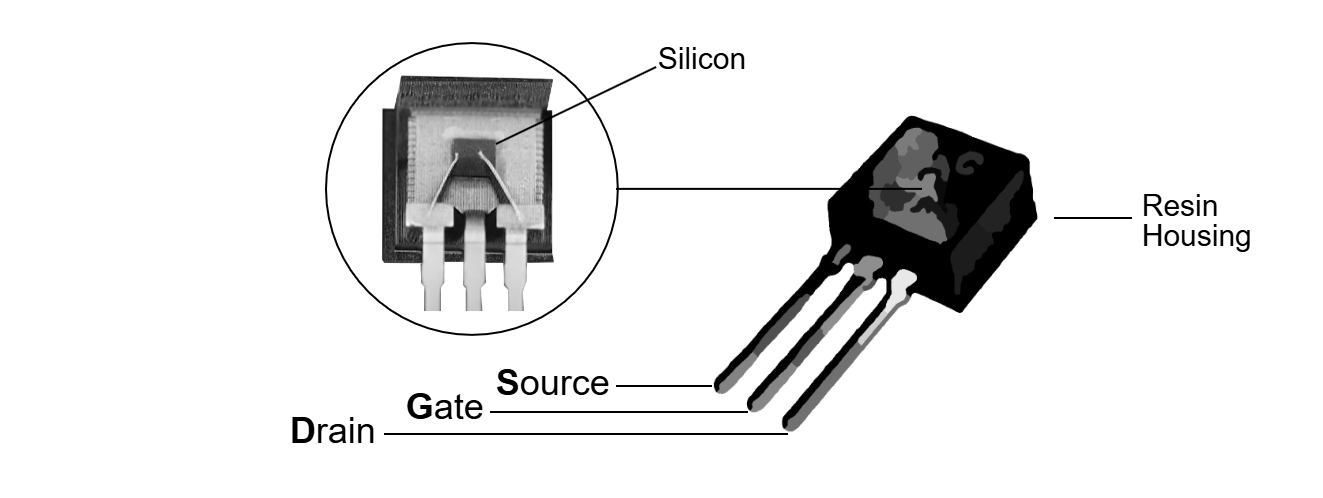
\includegraphics[width=\textwidth]{Sections/circuits/transistor.png}
  \caption{Cross-section of a discrete transistor: a silicon die (center) is bonded to three metal leads, all
    encased in an epoxy package.  A metal tab (not shown) may be added for heatsinking.}
  \label{fig:transistor}
\end{figure}

\newpage 



\begin{theo}[FETs over BJTs]

  \label{theo:why_mosfets_preferred}

  A BJT needs continuous base current, which wastes energy. A MOSFET only requires its gate to be charged or discharged (i.e., voltage applied or removed), which is more efficient.
\end{theo}

\noindent 
Now we briefly step into chemistry for completeness sake to understand differing silicon charges:
\begin{Def}[Anotomy of an Atom]

    \label{def:atom}

    An \textbf{atom} is the smallest unit of matter that retains the properties of an element. It consists of three main subatomic particles:
    \begin{itemize}
        \item \textbf{Protons:} Positively charged particles found in the nucleus.
        \item \textbf{Neutrons:} Neutral particles also found in the nucleus (same size as protons).
        \item \textbf{Electrons:} About the same charge as proton, but negative, and about 1800x smaller and lighter than a proton.
    \end{itemize}

    \noindent
    Protons and neutrons are tightly packed together in a space called the \textbf{nucleus}, gaining the name \textbf{nucleons};
    Electrons orbit the nucleus at discrete distances called \textbf{shells} or \textbf{energy levels}. 
    \underline{The number of protons in the nucleus defines the element (i.e., specifications).} E.g., 79 protons will 
    always be gold.

    Opposite charges attract, causing an \textbf{orbital space}, in which subatomic particles never collide (i.e., alike orbiting planets). Neutrons act as a buffer between protons (e.g., Silver is 
    stable with 60 or 62 neutrons, but unstable with 61). Atoms with different number of neutrons are called \textbf{isotopes}, latin for ``same place''.
    Electrons may jump between shells and atoms. If there is a greater number of electrons to protons, the atom is \textbf{negatively charged} (anions), otherwise it is \textbf{positively charged} (cations)
    \cite{crashcourse2013nucleus}.
\end{Def}

\begin{Def}[Periodic Table]

    \label{def:periodic_table}

    The \textbf{Periodic Table of Elements} organizes all known elements by the number of protons in their nuclei. This is called an \textbf{atomic number} (e.g., 
    gold's atomic number is 79). Elements are abbreviated from their latin translations (e.g., gold is \textbf{aurum}, AU, which means ``shining dawn'').
    There are 118 elements, with 80 being stable and the rest being unstable isotopes. Anything past 82 protons (lead) is 
    unstable, undergoing radioactive decay.
\end{Def}

\begin{Tip} The periodic table is complete, hence movies that claim ``we discovered a new element!'' truly deserve science-fiction as their defining genre.
\end{Tip}
\newpage 
\noindent
We'll stop with the chemistry dive after these next two critical definitions

\begin{Def}[Shell Capacities \& Valence Electrons]

    \label{def:valence_electrons}

    The first shell of any atom can hold up to 2 electrons, and the second 8. From 1-20 periodic elements, the third and fourth 
    shells can hold 8 and 2 respectively. A \emph{full} shell is considered \textbf{stable}, otherwise it is \textbf{unstable}.
    This arrangement of electrons within the shells is called the \textbf{electron configuration} (EC) of the atom.
    An EC is written as a n-tuple, starting with the inner-most shell (e.g., 2, 8, 8, 2 for calcium).

    
    The outer most shell is called the \textbf{valence shell}. An atom's \textbf{valency} (the number of electrons in the valence shell) determines whether a chemical reaction will occur.
     If an atom is stable (i.e., full valence shell), it will not react with other atoms.
    Unstable atoms \emph{strive} to become stable by either gaining, losing, or sharing electrons with other atoms \cite{infinitylearn2018concept}.
\end{Def}

\begin{Def}[Chemical Bonds -- Molecules \& Compounds]

    \label{def:chemical_bonds}

    The act of atoms joining together (e.g., sharing electrons, which is called a \textbf{covalent bond}), forms a \textbf{molecule}. 
    Concretely, a molecule is a merger of two or more elements. We use subscripts to denote the number of atoms in a molecule (e.g., H$_2$O is water, with two hydrogen atoms and one oxygen atom).
    \textbf{Compounds} are a subset class of molecules that consists only of two more more \textbf{different} elements (e.g., H$_2$O is a compound, but O$_2$ is not, as it only has one element, oxygen)  \cite{breslyn2013molecule}.
\end{Def}
\noindent
Now to what we've been waiting for:
\begin{Def}[Doping -- N-type \& P-type Silicon]

    \label{def:doping}

    Silicon has 14 atoms, with an EC of (2, 8, 4); Hence silicon is unstable. If we view silicon (Si) as a 3D lattice (a string of Si atoms in 3D grid),
    each Si atom will share its four valence electrons with it neighbors to become stable (covalent bonding). This creates a \textbf{silicon crystal}.\\

    \noindent
    Adding another element to the silicon lattice is called \textbf{doping}. We 
    are interested in two types of doping \cite{engineermindset2024mosfet}:
    \begin{itemize}
        \item \textbf{N-type:} When adding an element like phosphorus (P), EC of (2, 8, 5), is added to the silicon lattice, one electron goes unused after the covalent bonding. This free electron creates a \textbf{negative charge carrier} (hence N-type).
        \item \textbf{P-type:} Conversely, adding boron (B), EC of (2, 8, 3), creates a \textbf{positive charge carrier} (hence P-type), as boron won't be able to share an electron equal amongst all its neighbors, leaving a \textbf{hole} (an empty space where an electron could be) in the lattice.
    \end{itemize}
\end{Def}

\newpage 

\noindent 
Let's visualize what we've learned so far:

\begin{figure}[ht!]

  \centering
  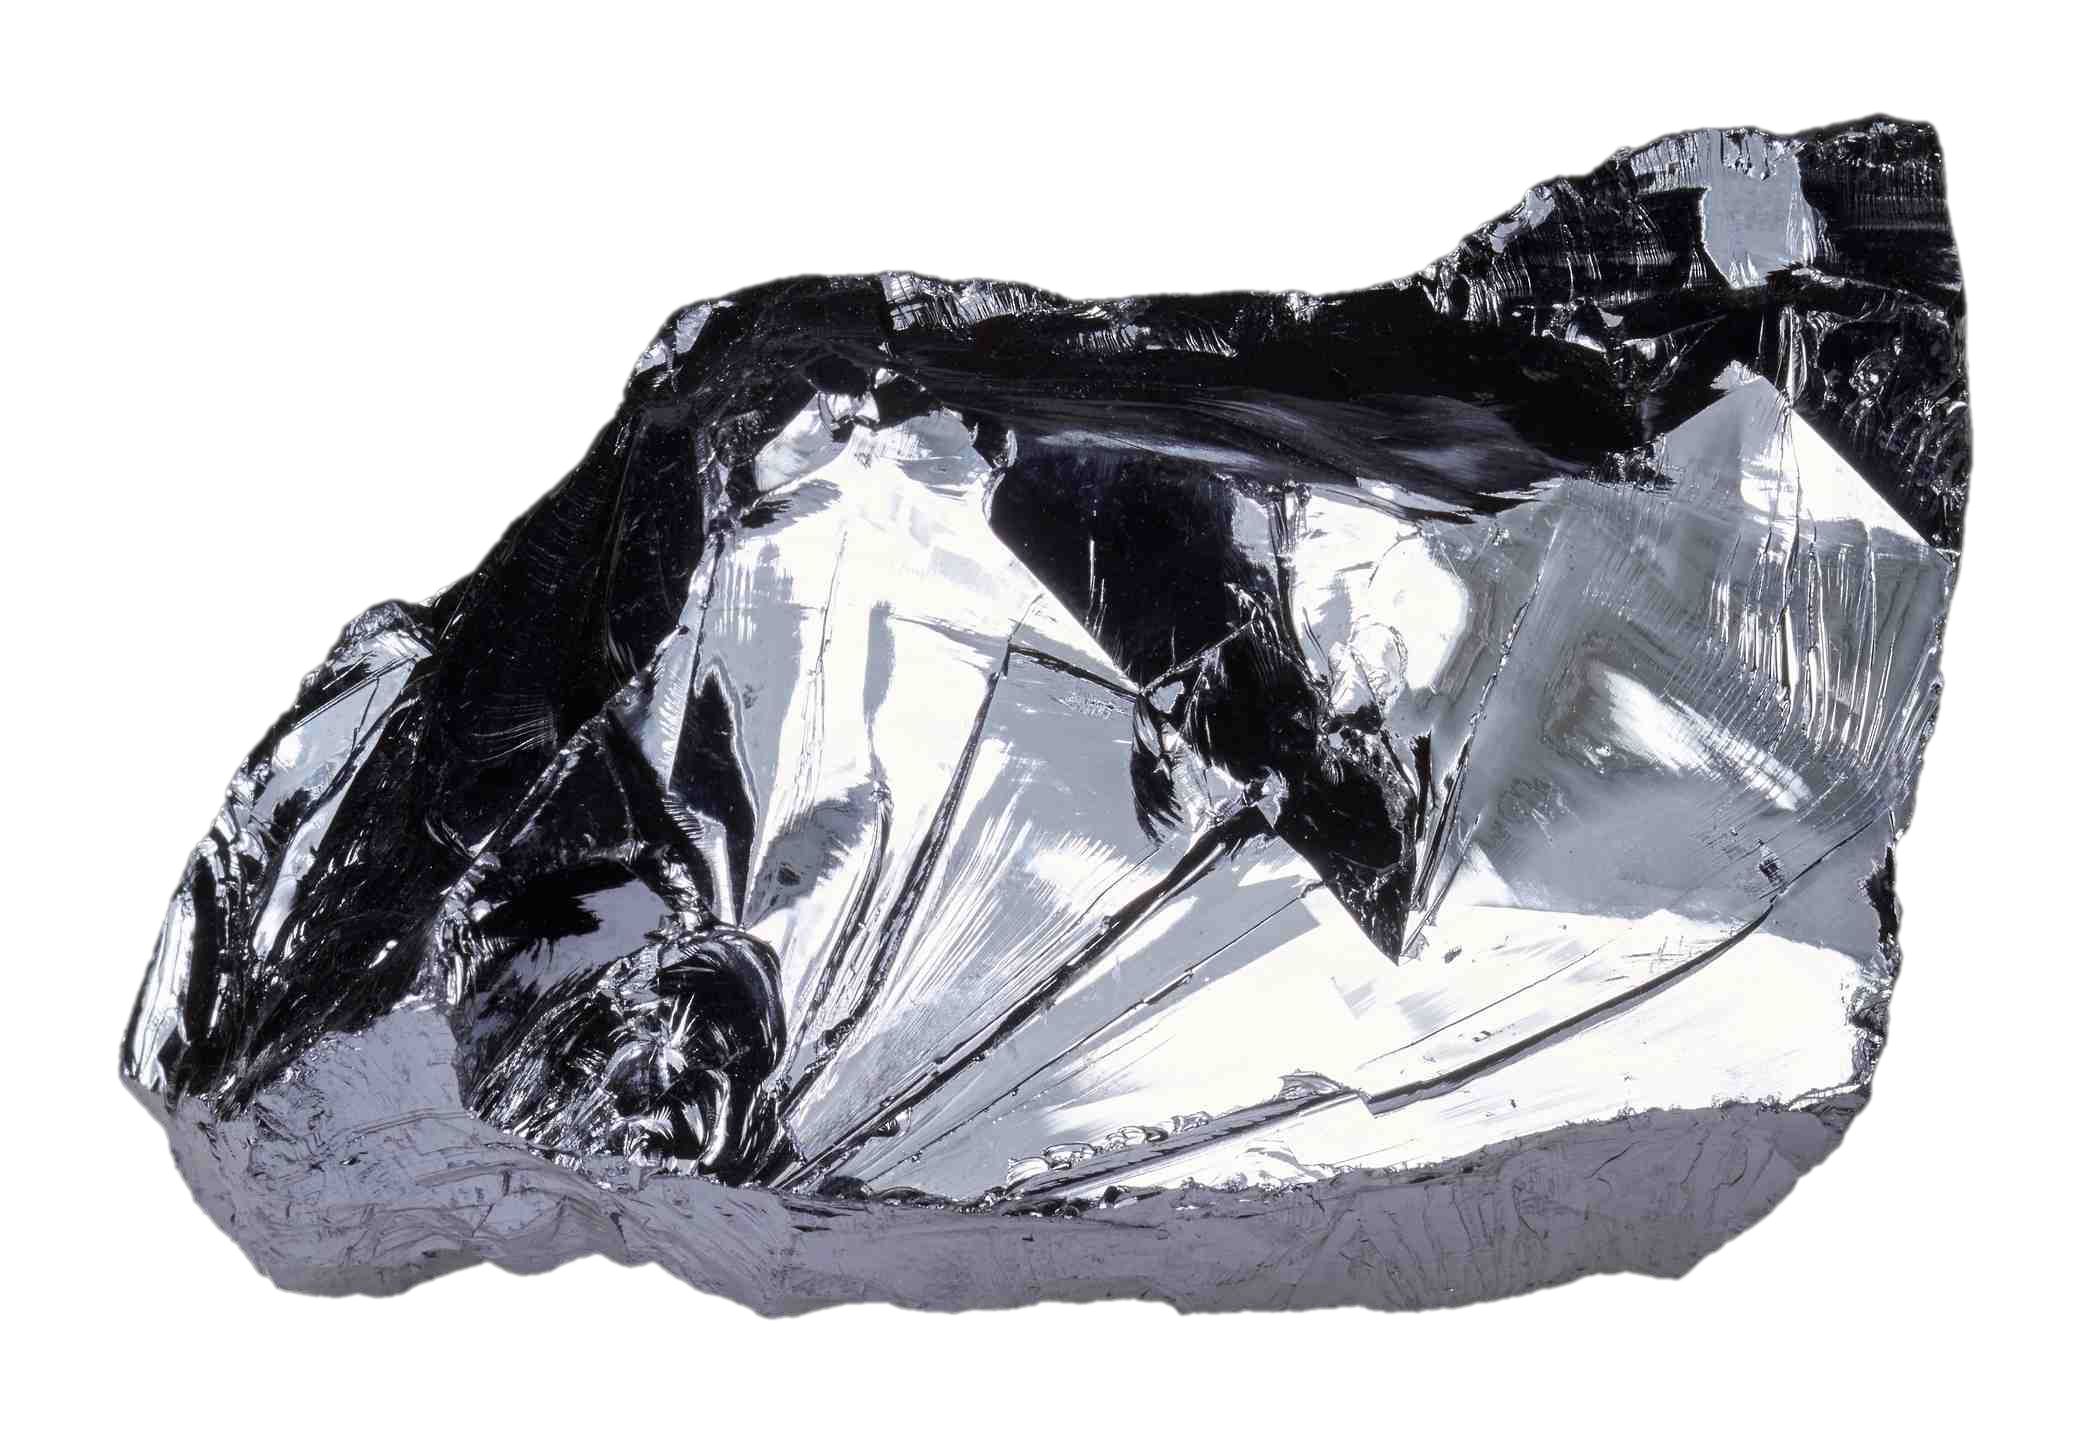
\includegraphics[width=.6\textwidth]{Sections/circuits/sicryst.jpg}
  \caption{An image of a silicon crystal \cite{gettyimages700832601}.}
  \label{fig:atom}
\end{figure}

\begin{figure}[ht!]

  \centering
  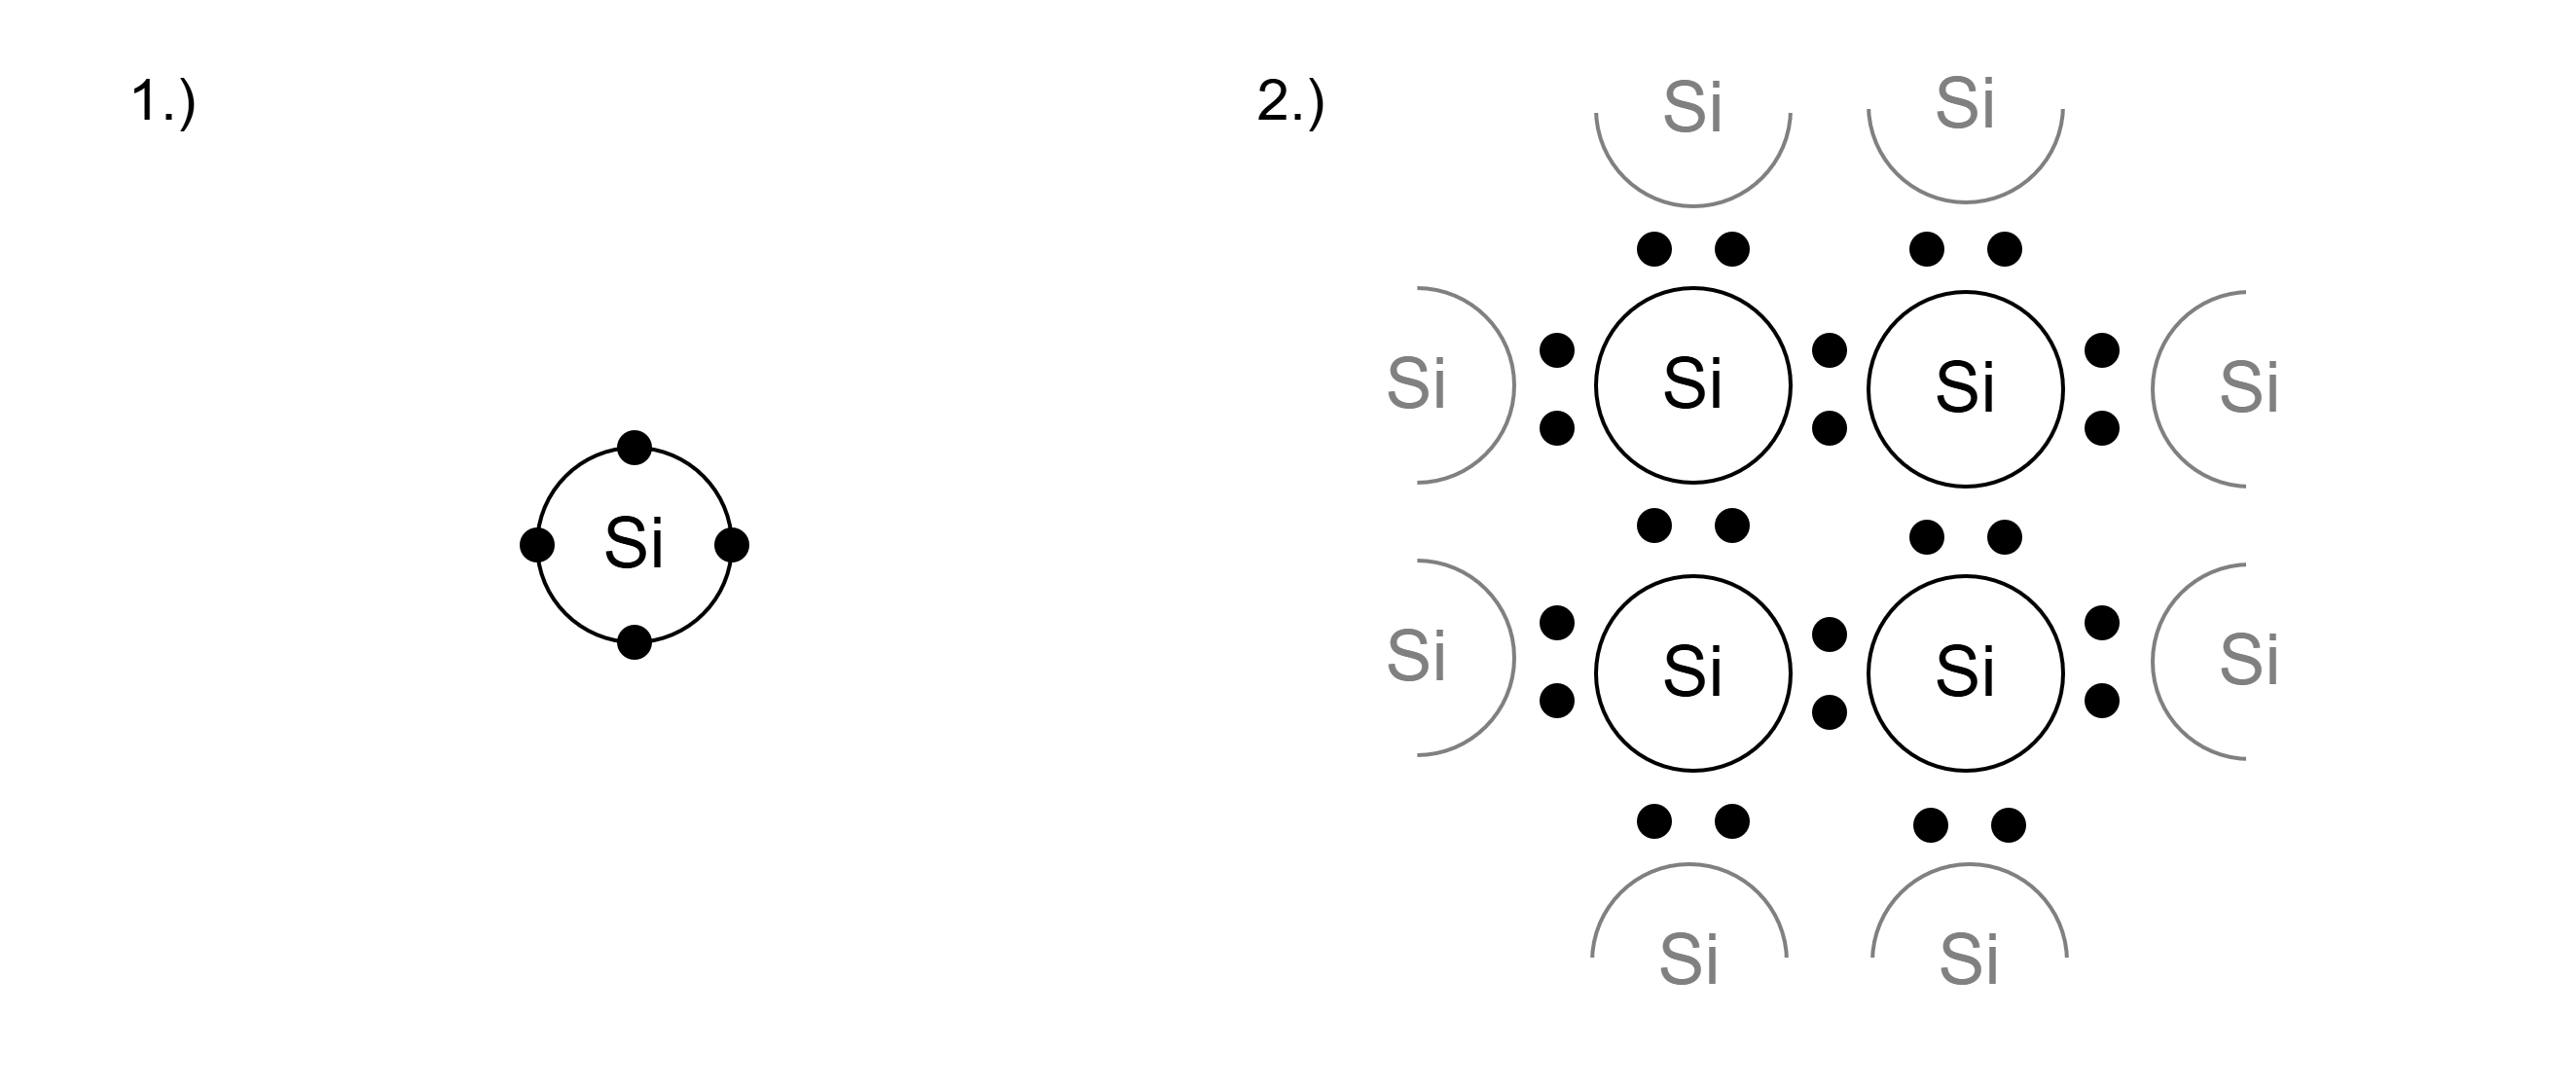
\includegraphics[width=\textwidth]{Sections/circuits/doping.png}
  \caption{(1) Shows a single silicon atom (Si) and its valence electrons (4 black dots).
  (2) Shows a flattened silicon lattice where neighboring Si atoms share their electrons to become stable.
  This creates an electron configuration of (2, 8, 8) for surrounded Si atoms.}
  \label{fig:doping}
\end{figure}
   
\newpage 

\noindent
\begin{figure}[ht!] 
  \centering
  \includegraphics[width=\textwidth]{Sections/circuits/doping2.png}
  \caption{(1) Shows a P-type silicon lattice, where boron (B) atoms are added, creating holes in the lattice.
  (2) Shows an N-type silicon lattice, where phosphorus (P) atoms are added, creating free electrons.}
  \label{fig:doping2}
\end{figure}
